\section{First Steps} \label{sec:FirstSteps}

Let's dive straight in and see Python in action. 

First we are going to launch the interactive Python environment, this requires us to get a command prompt. If you are on a windows computer then open a prompt from the start menu, alternatively if you are on Linux or a Mac you will run a terminal window. At the command prompt type \keyword{python} and you should see something like this:

\begin{center}
    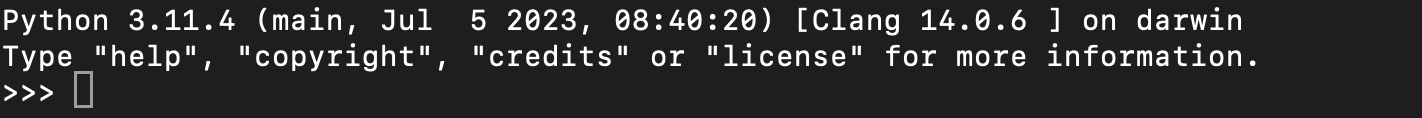
\includegraphics[width=1\linewidth]{images/screenshots/PythonEnv.png}
\end{center}

The number after the word Python tells you the version of the python language you are running. The only thing that matters for this book is that it starts with a number 3. The computer is now waiting for you to give it an instruction.  Try typing in each of these lines and press the return key after each line to see the result.

\begin{minipage}{\textwidth}
\lstinputlisting[language=Python,
    basicstyle=\sffamily\footnotesize,
    keywordstyle=\textbf, 
    commentstyle=\color{blue},
    showstringspaces=false,
    frame=tb, 
    numbers=none,  
    label={lst:PythonCode}]{Python/FirstCommands.py}
\end{minipage}


You can see that Python is working as a calculator but let's think a little more about what's going on here. When you press return Python is taking the characters you have typed and splitting it up into tokens it recognises, that is numbers and mathematical operators. We are limited in what we can type by the QWERTY keyboard we are using so we sometimes need to use special characters to tell Python what we need. For example line 2 means $5 \textsf{multiplied by} 6$ but there isn't really a multiplication symbol on our keyboard so we have to you the asterix (or star) symbol. Similarly $/$ means divided by and $**$ means to the power. 

Indeed Python has no real intelligence if it receives a command it understands then it does what it's told, if it receives something it doesn't understand then we get an error, such as we see with line 6. The error on this line is known as a $\textsf{Syntax Error}$. Put simply it means that the words used, or the way the sentence is constructed, is not understood by the computer (or Python in particular).  The error message provided tries to help us to see where we have gone wrong by telling us which line the error is on and pointing at the part of the line where the error exists.

\begin{center}
    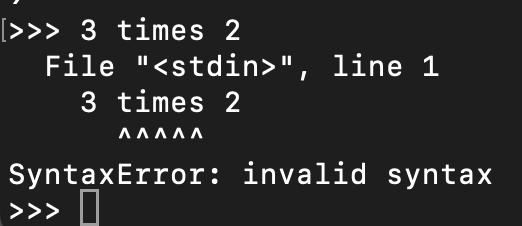
\includegraphics[width=0.3\linewidth]{images/screenshots/SyntaxError.png}
\end{center}

The final command we gave to Python, $\textsf{quit()}$ tells the interpreter to close.

\section{Your first Program}

In the previous section we saw how to give commands to Python, but each command was unrelated. Writing computer programs typically requires us to use multiple commands, in a predefined order, to accomplish a task. This set of commands is called a computer program and, in this section, we will write our first program. This will require us to make use of a program editor and, in our case we are going to use Microsoft Visual Studio Code. I chose this editor because it's available for all computing platforms (there is even a web version and one for Raspberry pi computers).

So let's get started and launch Visual Studio Code. Create a new file and call it \keyword{my\_first\_program.py}. You might want to create a folder on your computer to store your programs from the book. The reason we give teh program the extension ``.py'' is so that the computer knows this is a python file.

Because we are using Visual Studio Code and it knows what a python file so, if you haven't yet installed the python extensions to the editor, you will asked if you'd like to, please go ahead and do so, it might take a few minutes. Now type in the following program. If you understand what the program is doing then great, if not then don't worry we will learn what it means through the rest of the book.

\begin{minipage}{\textwidth}
\lstinputlisting[language=Python,
    basicstyle=\sffamily\footnotesize,
    keywordstyle=\textbf, 
    commentstyle=\color{blue},
    showstringspaces=false,
    frame=tb, 
    numbers=none,  
    label={lst:PythonCode}]{Python/FirstProgram.py}
\end{minipage}

Now save your program and look from the Triangle at the top of the screen this is the \keyword{Run Python File} button.

\begin{centering}
    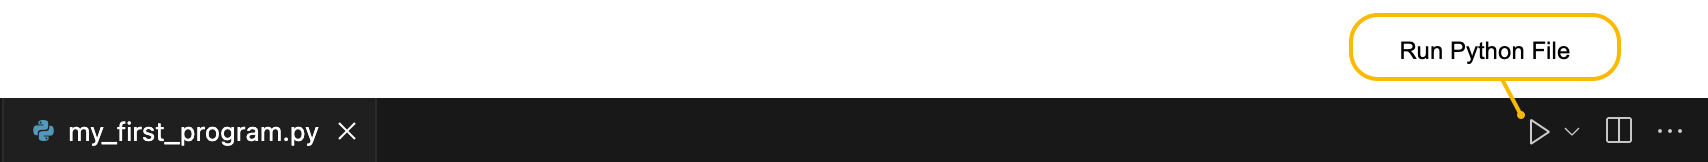
\includegraphics[width=1.0\linewidth]{VSCode-Run.png}
\end{centering}

When you press this button you are telling VSCode to send your commands to the python interpreter. VSCode then opens a new window which contains a command window, just like the one you used earlier, and calls python passing it the file you created. You can see the output created by your file in the bottom window as seen below. Don't worry if your editor looks slighly different to this VSCode allows you to change colours and icons to suit your preferences. We won't spend much time looking at this here but you might want to explore the editor more by visiting the visualstudio website : \url{https://code.visualstudio.com/docs/introvideos/basics}.

\begin{center}
    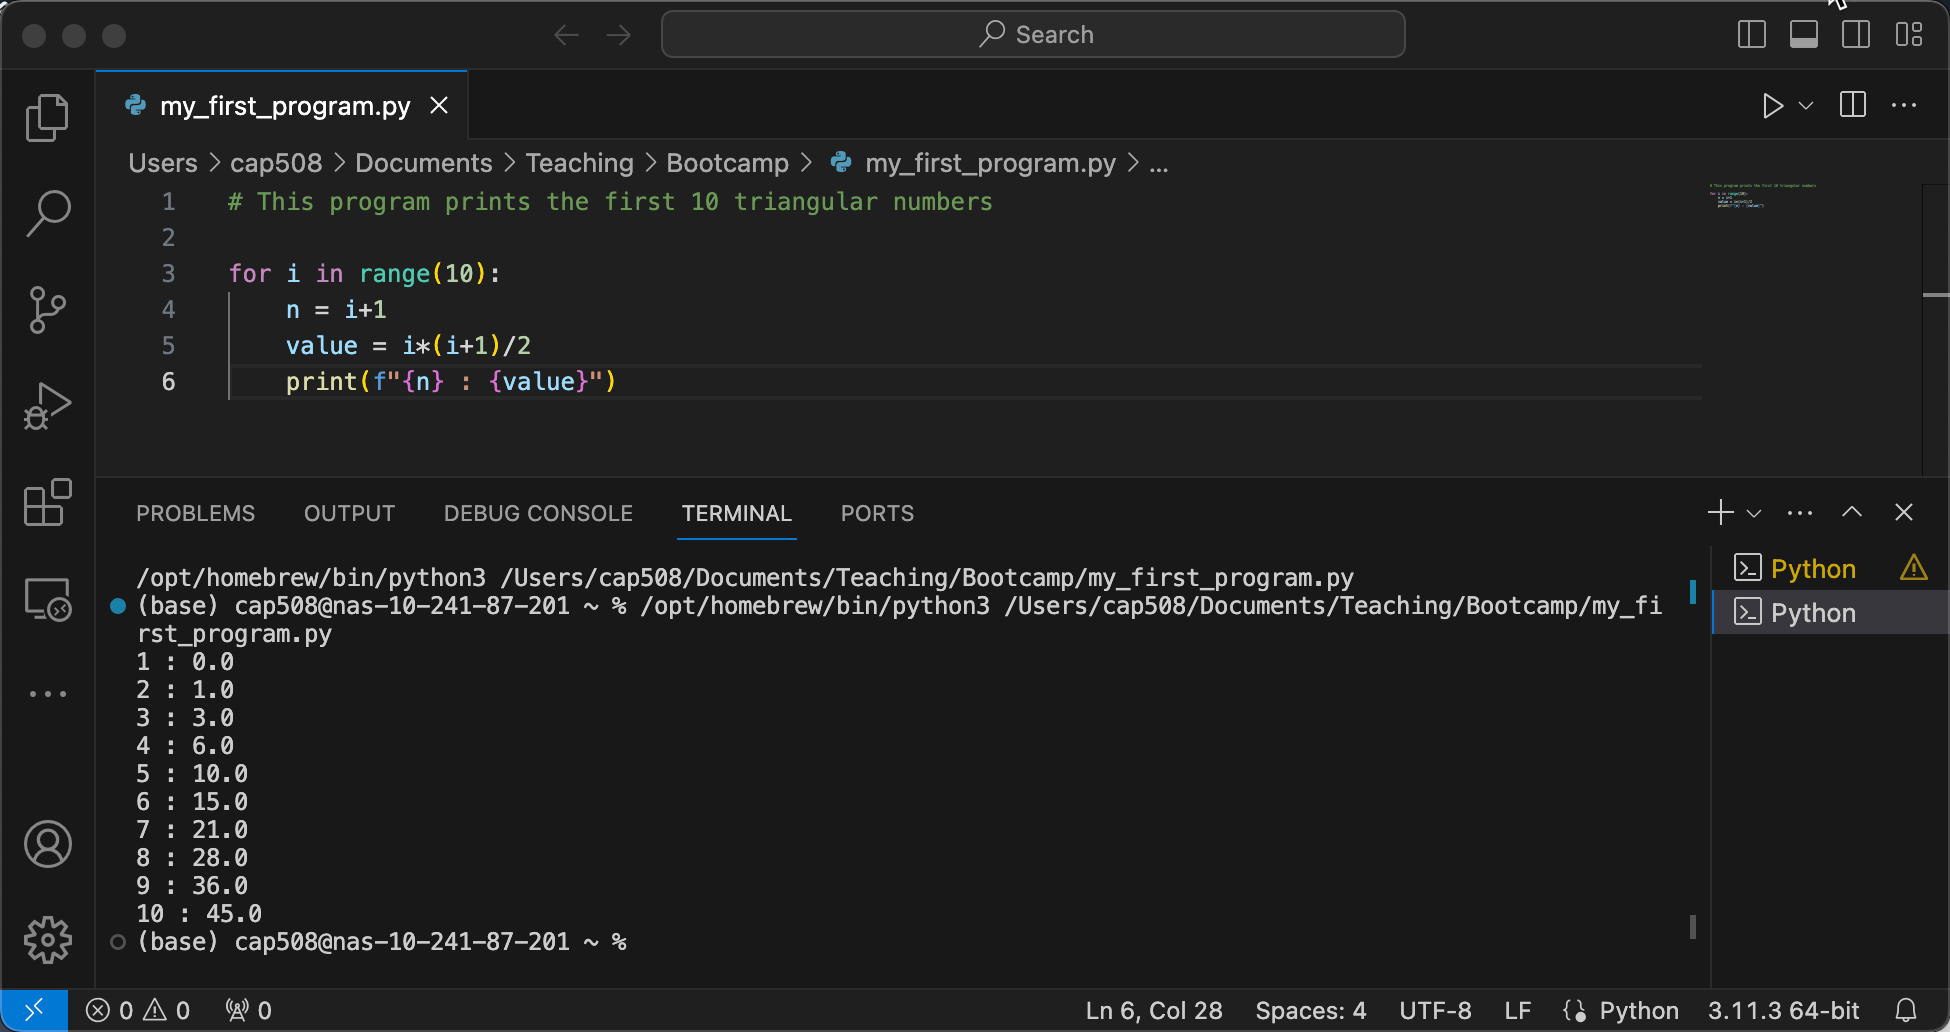
\includegraphics[width=1.0\linewidth]{images/screenshots/VSCodeEnv.png}
\end{center}

Well done. You've started your programming journey. In the next section we are going to learn the basics ideas which are common to many different programming languages and see how we create and manipulate data using Python.

%Resources and helpful links
% it might be worth creating a useful links and addtional reading section. 
%

